\subsubsection{Cittadino esperto}
\label{sss:citadino-esperto}
\begin{wrapfigure}{r}{8cm}
    \vspace{-13pt}
    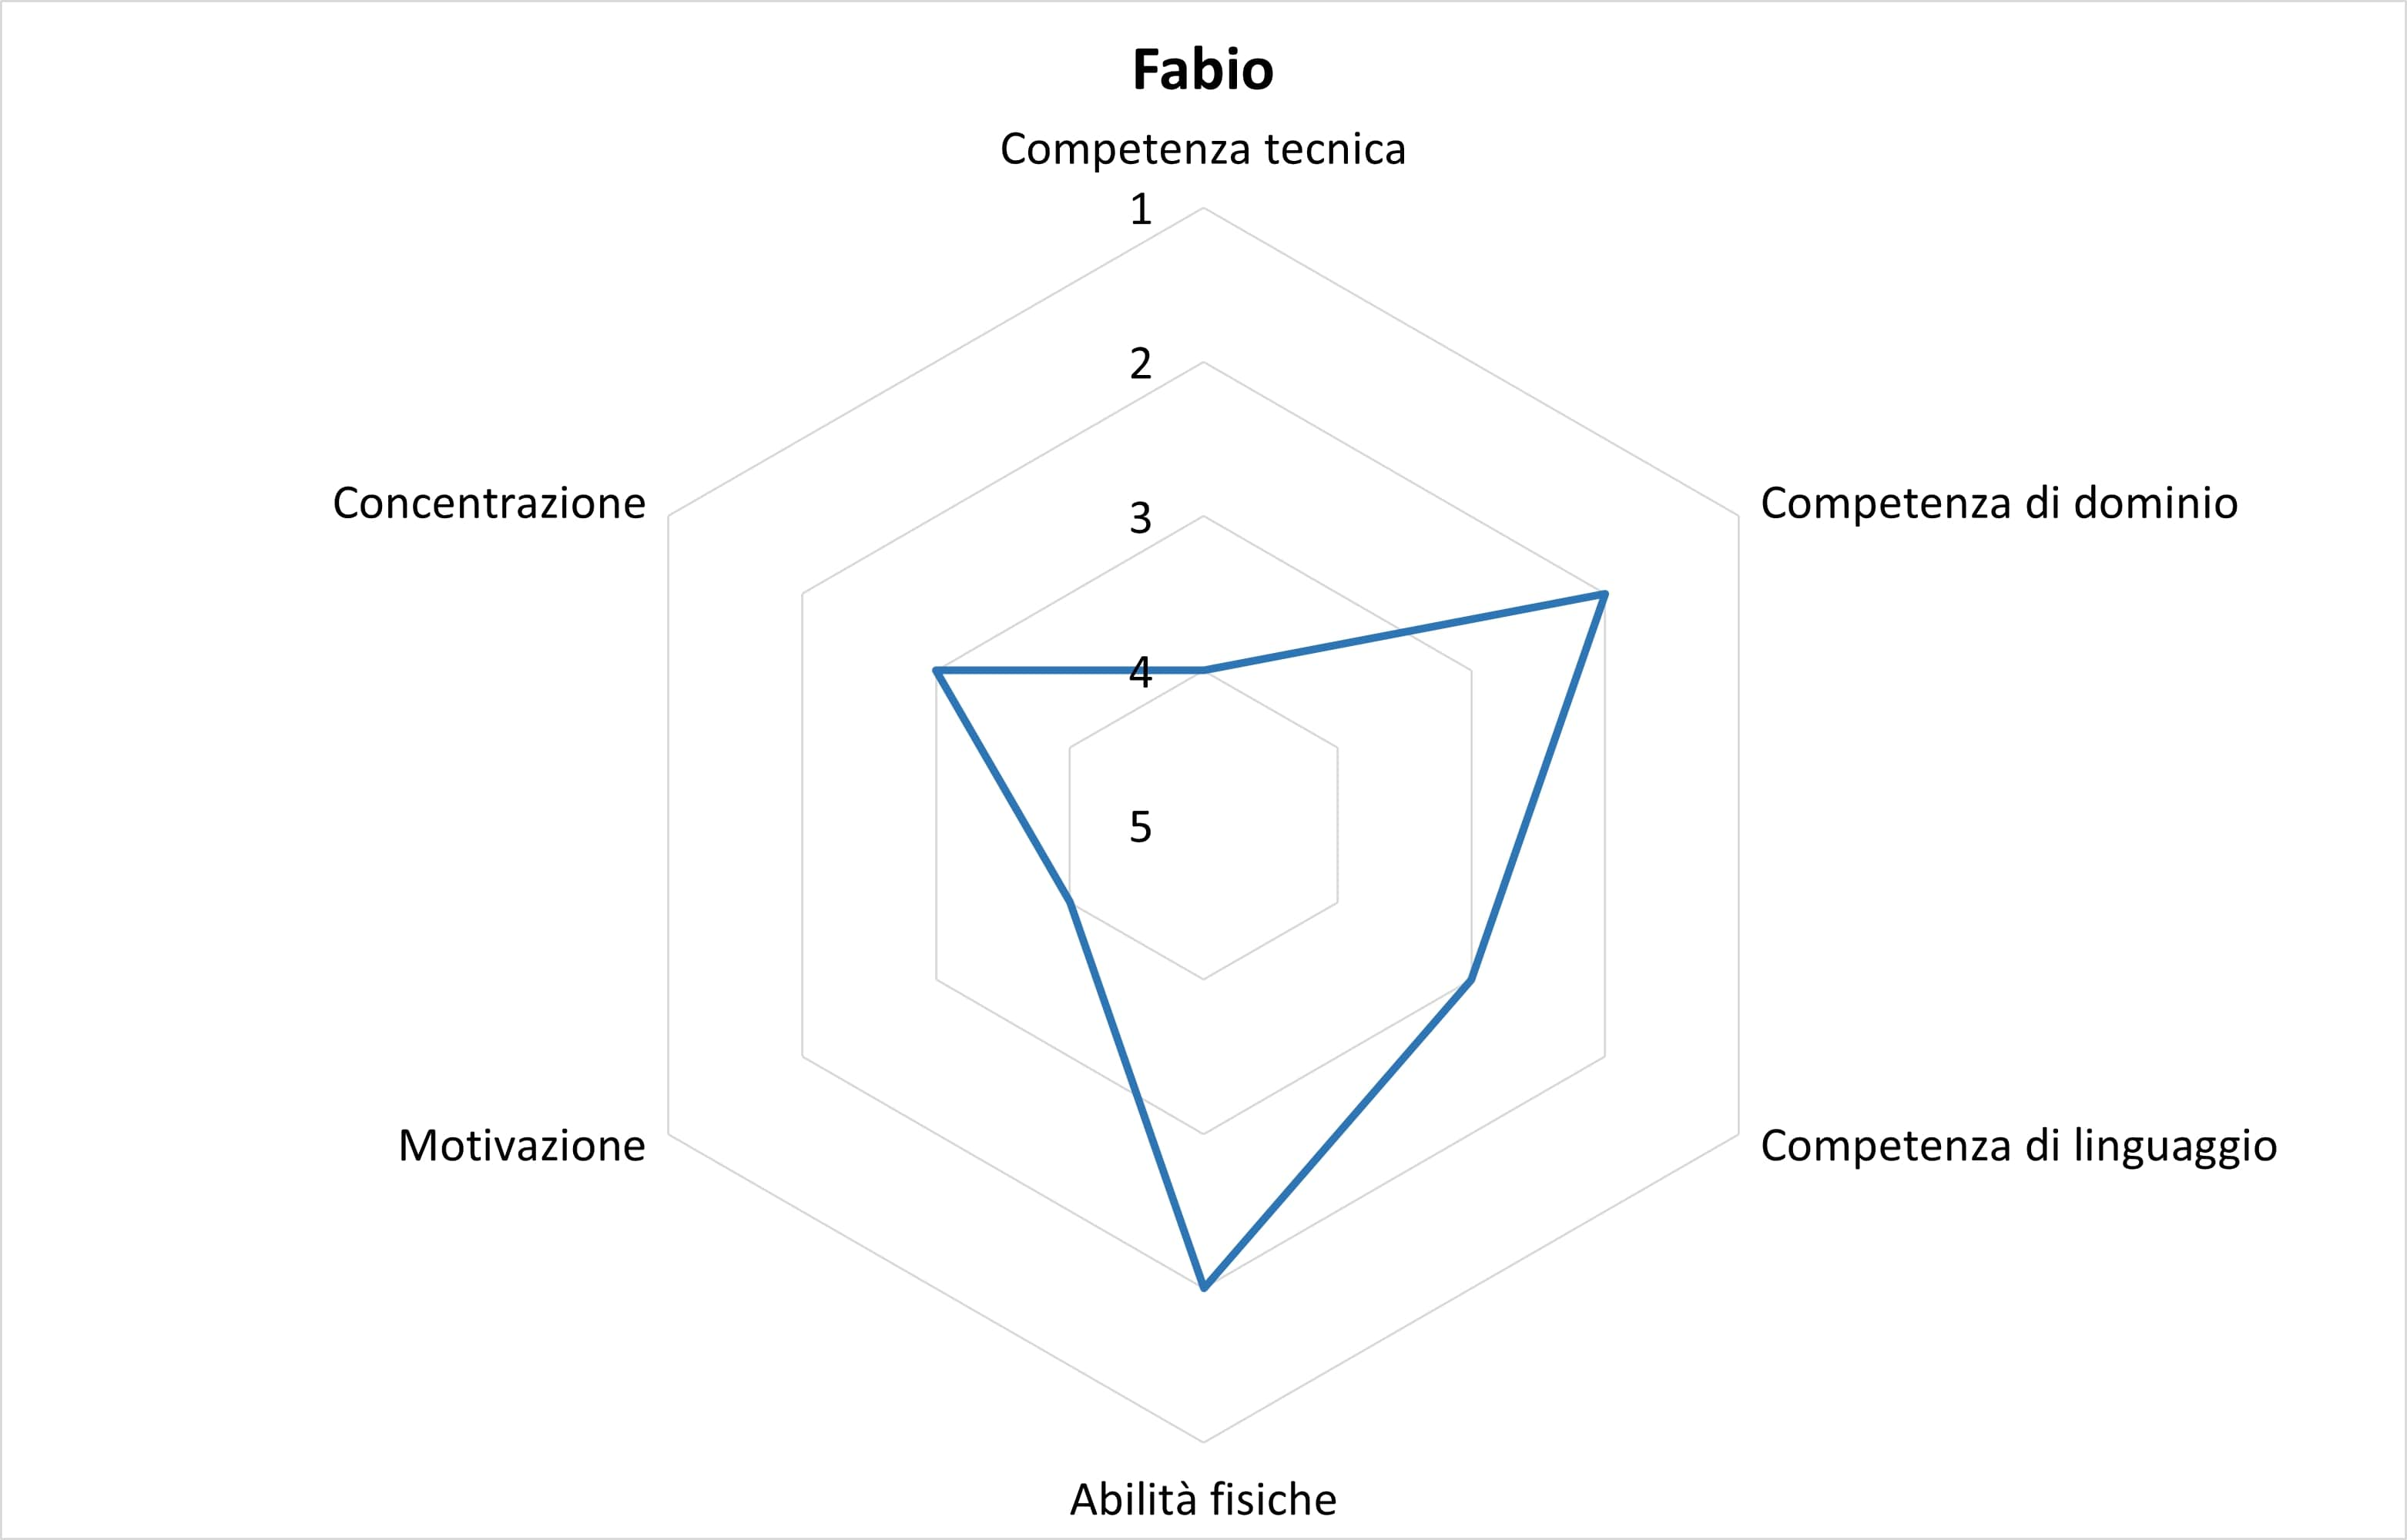
\includegraphics[scale=1.5]{studio-fattibilità/fabio}
    \caption{Foto fantasiosa della persona Fabio}
    \vspace{-13pt}
\end{wrapfigure}
Fabio è un uomo di 62 anni del Pescarese, la cui quotidianità è illuminata dalla sua famiglia e dal suo lavoro come docente universitario di Informatica presso l'Università degli Studi G. D'Annunzio (Chieti-Pescara).\\ 
È sposato da 25 anni con Claudia, infermiera presso l'Ospedale S. Spirito di Pescara ed è padre di un'adolescente di 17 anni e un giovane di 23 anni: una delle abitudini più preziose della famiglia di Fabio è la condivisione della cena, durante la quale si parla delle attività di ognuno e si intavolano riflessioni circa le ultime notizie dall'Italia e dal mondo.\\
Negli anni, Fabio ha cercato di trasmettere ai figli il profondo rispetto che riconosce alle istituzioni, oltre alla fiducia che ripone nella scienza. Inoltre, è molto sensibile al dilagare delle fake news nei diversi ambiti: crede che siano responsabili di una cattiva informazione delle persone, e quindi di una loro consapevolezza distorta della realtà.\\ 
Queste sue considerazioni emergono non solo in famiglia ma anche nei momenti di svago, ad esempio durante le chiacchierate con gli amici.\\ 
Ogni giorno, Fabio cerca di informarsi tramite canali considerati attendibili e autorevoli; negli ultimi mesi imperversati dalla pandemia Covid-19, ha esteso il suo briefing mattutino anche alla dashboard del DPC: grazie alle sue competenze informatiche, riesce a consultarla in maniera agevole. In particolare, vi si rivolge quando gli articoli di giornale che legge si rivelano confusionari o non allineati: la dashboard, presentando dati in maniera immediata e chiara, permette a Fabio di dirimere i dubbi e acquisire l'essenziale; di frequente, estrae elementi grafici dalla dashboard per poi condividerli con i contatti dei suoi social, a corredo di proprie riflessioni.
\begin{itemize}
	\item Attitudine:
    \begin{itemize}
        \item vuole maturare una propria opinione sugli argomenti di attualità;
        \item vuole contribuire ad un'informazione sana e corretta dei suoi familiari;
        \item ragionevole e responsabile, incline al rispetto delle istituzioni, fiducioso nella scienza;
    \end{itemize}
	\item Comportamento: 
    \begin{itemize}
        \item connessione alla dashboard sporadica, solo quando ha necessità di informarsi o ha ritagli di tempo libero;
        \item condivide e discute circa le informazioni acquisite con colleghi e amici;
    \end{itemize}
    \item Obiettivi (\textit{end goals}): integrare quanto letto presso articoli di giornali di varia natura;
    \item Motivazione (\textit{life goals}): acquisire maggiore consapevolezza e conoscenza dei fenomeni che impattano la realtà in cui vive, nonché la capacità di discernere l'essenziale dal \textit{mare magnum} di informazioni che, continuamente, lo investono;
    \item Obiettivi del sistema:
    \begin{itemize}
        \item filtro per regione;
        \item estetica accattivante e grafici interattivi.
    \end{itemize}
\end{itemize}